\documentclass[a4, 12pt]{article}
\usepackage{graphicx}
\usepackage{hyperref}
\usepackage{datatool}
\usepackage{apacite}
\usepackage{dingbat}
\usepackage{subcaption}
\usepackage{wrapfig}
\usepackage{amsmath}
\usepackage{placeins}
\usepackage{caption}
\usepackage{threeparttable}
\usepackage{ragged2e}
\usepackage{hyperref}
\usepackage{natbib}
\usepackage{pdflscape}

\hypersetup{
    colorlinks=true,
    allcolors=cyan
}
\newcommand{\citeg}[1]{\citep[e.g.][]{#1}}
\newcommand{\fref}[1]{(Figure \ref{#1})}

\title{Geophysically constrained inversions of glacier bed topography \\
 \large Resume of an USRA project}
\author{Alexi Morin}


\begin{document}
\maketitle
\section{Introduction}
\subsection{Motivation}
Inferring glacier thickness has been a long-standing problem for glaciologist. Determining mean ice thickness lets us estimate the total volume of ice in a given glacier, necessary to quantify the water stored. In the context of climate change, a proper estimate of ice thickness is necessary for correctly estimating sea-level change \citeg{farinotti2016accurate}. Many techniques have been developed for this problem, such as \textit{power laws} or \textit{scaling methods}, deriving total ice volume from glacier surface area \citep[e.g.][]{bahr2015review}. However, the development of more precise runoff projections \citeg{ramsankaran2018spatially} and glacier flow models \citeg{werder2020bayesian} is asking for distributed ice thickness information.\\

Acquiring such data today is often done with a sled-mounted or airborne ground penetrating radar (GPR). While airborne surveys are very effective on ice caps and ice sheets, the complications following the processing of the data in mountainous areas poses another difficulty. Furthermore, ground based surveys can  be a very challenging feat as traversing highly crevassed areas is on its own complicated let alone while hauling heavy equipment. \citeg{colombero2019ice} Those ground surveys can then often leave out vast unmeasured areas, forcing the scientist to extrapolate the acquired data. These reasons motivate the development of physical and statistical ice thickness inference models. \\

These methods, using theoretical and mathematical models, often rely on assumptions such as uniform basal shear stress and require additional information such as an estimation of basal velocity \citeg{farinotti2016accurate}. The number of models is rapidly increasing, hence the need for evaluations of their performance under various conditions. The Ice Thickness Models Intercomparison eXperiment \citeg{farinotti2016accurate} \textit{ITMIX} called for a total of 17 models applied to 21 study sites. This study was the basis for the development of a global estimate of distributed glacier thickness \citeg{farinotti2019consensus}. The five best performing models from the experiment needing easily available satellite data were used to make this worldwide estimation. The model outputs are freely available online for glaciers included in the Randolph Glacier Inventory \citeg{pfeffer2014randolph}.\\

The first objective of this project is to assess the accuracy of the ice thickness distribution inferred from \citet{farinotti2019consensus} and other available  models at five study sites of interest to the SFU Glaciology Group. As there is little GPR coverage for our two main study sites, the models will also be compared for two other sites where the bed topography is better known.\\
The second objective is to produce an improved model of the ice-thickness distributions based on the comparison of the ITMIX output and various models and in-situ ice-thickness measurements. The different methods explored by \citeauthor{farinotti2019consensus} in \textit{ITMIX} are detailed and information about the necessary data for every method is presented. A review of every study sites explored in this project is presented, followed by the assessment of the error in the consensus estimate\citeg{farinotti2019consensus} and other models by comparing them to in-situ data.

\section{Background}
\subsection{\textit{ITMIX}}
The Ice Thickness Models Intercomparison eXperiment \citep{farinotti2016accurate} is a project launched by the Working Group on Glacier Ice Thickness Estimation, part of the International Association of Cryospheric Sciences (IACS).
The experiment consists of 17 different models tested over 21 cases.Every glacier in the comparison however had at least:
\begin{itemize}
\item a glacier outline (\textbf{GO}) 
\item a digital elevation model (\textbf{DEM})
\end{itemize}
And a combination of:
\begin{itemize}
\item the surface mass balance (\textbf{SMB})
\item the velocity field ($\boldsymbol{\vec{V}}$)
\item the rate of ice thickness change ($\boldsymbol{\frac{\partial h}{\partial t}}$)
\end{itemize}
% Need to get the actual sources for these
Four main types of models were outlined throughout the experiment, each needing specific data.
\begin{itemize}
	\item Minimization approaches
		\begin{itemize}
			\item Those models defines ice thickness inversion as a minimization problem. They use a cost 					function consisting of minimizing the difference between observed and modelled data. 	
		\end{itemize}
	\item Mass conserving approaches
		\begin{itemize}
			\item These methods are based on the principle of mass conservation 												\cite{farinotti2016accurate} The ice flux divergence $\nabla \cdot q$ has to be compensated by the rate of ice thickness change $\frac{\partial h}{\partial t}$ and the climatic mass balance $ \dot{b}$:
					\begin{equation}
						\nabla \cdot q = \frac{\partial h}{\partial t} - \dot{b},
					\end{equation}
		\end{itemize}
	\item Shear-stress based approaches
		\begin{itemize}
			\item Those approaches rely on some estimation of the basal shear stress $\tau$. They then 					solve for the ice thickness $h$ using the shallow ice approximation (Fowler and Larson, 1978)
			\begin{equation}
					h = \frac{\tau}{f\rho g \sin{\alpha}} % Is it really??? Correct source
			\end{equation}
			where $\rho$ is the ice density, $g$ is the gravitational acceleration, $\alpha$ the slope 					angle and $f$ is a friction coefficient.
		\end{itemize}
	\item Velocity-based approaches
		\begin{itemize}
			\item The models described in this category are based on a form of Glen's flow law \citeg{glen1958flow} and an approximation of either the basal velocity $u_b$ or the depth-averaged  				velocity $\bar{u}$ from the surface velocity $u_s$.
		\end{itemize} 
	\item Other approaches
		\begin{itemize}
			\item GCneuralnet\citep{clarke2009neural} is a model based on artificial neural networks. It is based on the assumption that the subglacial topography resembles nearby unglacierized valleys.
			\item The method from Brinkerhoff \citep{brinkerhoff2016bayesian} is based on Bayesian inference. The idea is that the bed elevation and the ice flux divergence can be described as Gaussian random fields with known covariance but unknown mean.
		\end{itemize}		
\end{itemize}
The requirements of each of the main mode types are shown in table \ref{tab:itmix_models}. 
\begin{table}[h!]
	\centering
	\caption{Models compared in \textit{ITMIX}. A checkmark with an asterix means that the model can make use of the data but it is not needed. Note that the table indicates the needs of the majority in the models presented, some models in the category use more or less data than shown in the table. Further information is shown in \citet{farinotti2016accurate}.} \label{tab:itmix_models}
	\begin{tabular}{|c|c|c|c|c|c|}
	\hline
	Model&\textbf{GO}&\textbf{DEM}&\textbf{SMB}&$\boldsymbol{\vec{V}}$&$\boldsymbol{\frac{\partial h}{\partial t}}$\\
	\hline
	Minimization approach & \checkmark & \checkmark & \checkmark & \checkmark * & \\
	\hline
	Mass conservation approaches & \checkmark & \checkmark & & & \\
	\hline
	Shear-stress based approaches & \checkmark & \checkmark & & & \\
	\hline
	Velocity based approaches & \checkmark & \checkmark & & \checkmark & \\
	\hline
	GCneuralnet & \checkmark & \checkmark & & & \\
	\hline
	Brinkerhoff & \checkmark & \checkmark & \checkmark & \checkmark & \checkmark \\
	\hline
	\end{tabular}
\end{table}
\\
\textit{ITMIX} ranked the models from best to worst according to four error metrics:
\begin{itemize}
\item Average \item Median \item Interquartile range \item 95\% confidence interval
\end{itemize}
and over two rankings:
\begin{itemize}
	\item Their performance over the glaciers tested by every model. Here the models are compared only by the error metrics on the individual test cases.
	\item Their performance over all the glaciers. Here the models are penalised for a smaller number of cases tested.
\end{itemize}
One of the main conclusions from \textit{ITMIX} is that the models needing more sophisticated data, such as the velocity fields $\boldsymbol{\vec{V}}$, surface mass balance $\boldsymbol{SMB}$ or $\boldsymbol{\frac{\partial h}{\partial t}}$ do not necessarily yield a better model. The inconsistencies between the available datasets, often acquired using different methodologies appears to be the cause \citep{farinotti2016accurate}. As there are limited data available for our study sites, it is important to choose a model corresponding to potentially available data for our study cases. The findings of \textit{ITMIX} confirms that the lack of $\boldsymbol{\vec{V}}$ or $\boldsymbol{\frac{\partial h}{\partial t}}$ data should not gravely impact the inferring process for our test cases if such data was not available.
\section{Study sites}

\subsection{North Glacier}

\begin{figure}[h!]
\centering
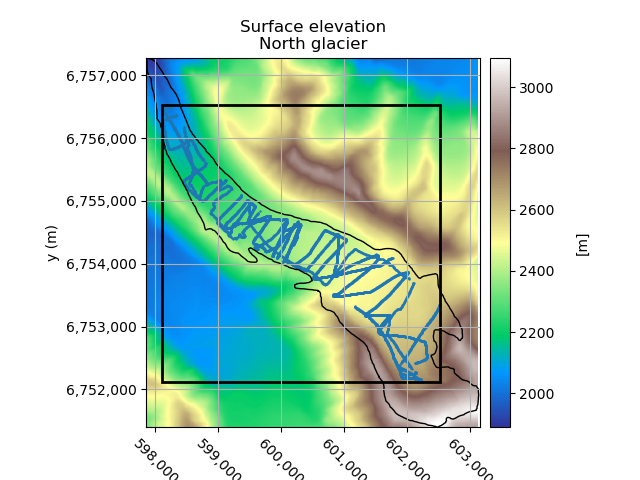
\includegraphics[scale=0.8]{../imgs/North glacier/elevation.png}
\caption{Surface elevation (Need etienne citation) of North Glacier and surroundings with coverage of ice-penetrating radar measurements (red outline). Black outline from \citet{pfeffer2014randolph}}
\label{fig:ng_dem}
\end{figure}
\subsubsection{Site description}

North Glacier, located in the St. Elias mountains, was extensively studied by Flowers and her team between (???). This relatively small glacier, spanning 6.9\,km$^2$, is well known, with a GPR coverage of 4.89\,km$^2$ (Figure \ref{fig:ng_dem})\footnote{GPR coverage polygons were computed as the intersection of the glacier's outline and the convex hull delimited by the GPR point data}. Many data sets are available for this glacier, making it a great tool for testing techniques.

\subsubsection{Data available}
Surface elevation data available for this glacier are two 20\,m resolution DEM from \citet{berthier2008spot5} and (Need citation from Etienne, see july 10 email), with time-scales representing 2007 and 2018 respectively. From this data was produced a surface elevation change raster, with the same 20\,m resolution. 240\,m resolution surface velocities from 1985 to 2018 are available from ITS\_LIVE \citeg{gardner2019its_live} and 20\,m resolution surface velocities from 2018 are available from (Need etienne's citation). Finally, ice thickness measurements from 2008 are available. 
\subsection{South Glacier}

\begin{figure}[h!]
\centering
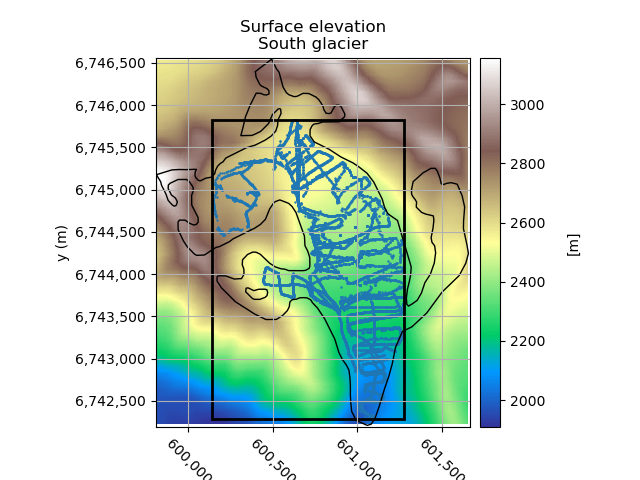
\includegraphics[scale=0.8]{../imgs/South glacier/elevation.png}
\caption{Surface elevation (Need etienne citation) of South Glacier and surroundings with coverage of ice-penetrating radar measurements (red outline). Black outline from \citet{pfeffer2014randolph}}
\label{fig:sg_dem}
\end{figure}

\subsubsection{Site description}
South Glacier was also extensively studied in the same period as North Glacier's. This smaller 5.65\,km$^2$ glacier shows a great GPR coverage of 3.81\,km$^2$ (\ref{fig:sg_dem})

\subsubsection{Data available}
Apart from the GPR measurements, 20\,m resolution data DEM and surface velocities from 2018 (Need étienne citation) are available.

\subsection{Kaskawulsh Glacier}
\begin{figure}[h!]
\centering
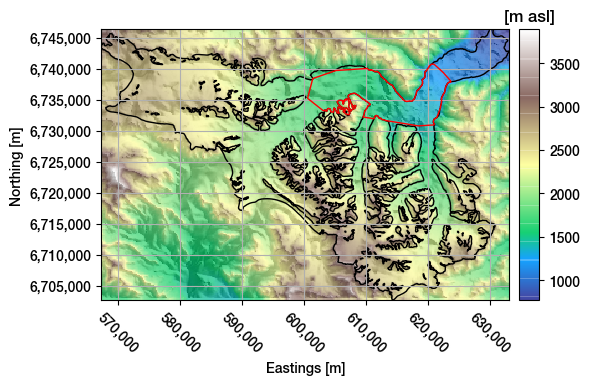
\includegraphics[scale=0.8]{../imgs/Kaskawulsh glacier/elevation.png}
\caption{Surface elevation \citep{farinotti2019consensus} of Kaskawulsh Glacier and surroundings with coverage of ice-penetrating radar measurements (red outline). Black outline from \citet{pfeffer2014randolph}}
\label{fig:sg_dem}
\end{figure}
\subsubsection{Site description}
Kaskawulsh Glacier is a considerably large glacier of 1053.16\,km$^2$ in the St. Elias mountains. This glacier was studied by Ph.D. student Erik Young as part of a mass balance research project. GPR transects were acquired during the summers of 2018 and 2019, covering approximately 127.84\,km$^2$.
\subsubsection{Data available}
Ask Erik about the DEMs used for this particular glacier. None were really used in the process however. More work here is needed.

\subsection{Job Glacier}
\subsubsection{Site description}
% I think I need more information on the location and the history of the place. I'll go further into detail by reading more of Tryggvi's thesis proposal.
\begin{figure}[h!]
\centering
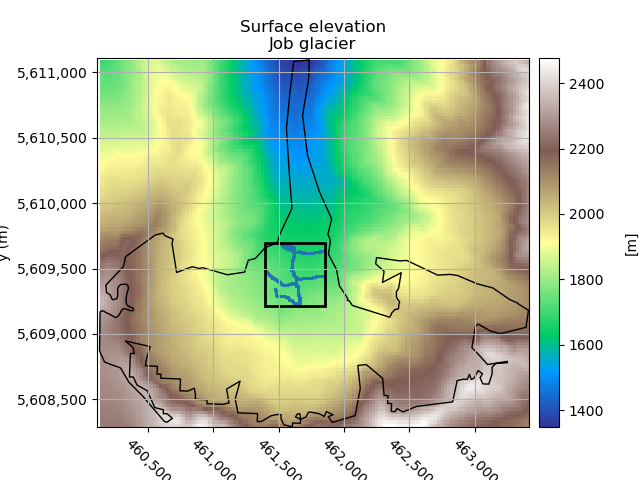
\includegraphics[scale=0.8]{../imgs/Job glacier/elevation.png}
\caption{Surface elevation of Job Glacier from \citet{roberti2018landslides} and surroundings with coverage of ice-penetrating radar measurements (red outline). Black outline from \citet{pfeffer2014randolph}}
\label{fig:job_dem}
\end{figure} % Is the landslide section pertinent? I understand that it is not in Tryggvi's main research focus, but it helps motivating the glacier flow model and the ice thickness
Job Glacier is a 3\,km long glacier covering $\sim$3\,km$^2$ located in the Mt. Meager complex, a volcano in southwestern British Columbia. This glacier, like most glaciers across the world, has seen a net negative mass balance in the last ten years \citep{reyes2004stratigraphic}. Fumaroles emerged from the surface of the glacier in 2016. \citet{roberti2018landslides}  states that the fumarolic activity has probably been active for a long period, but only recorded from the thinning of the glacier.
MSc research being undertaken by Tryggvi Unnsteinsson aims to understand the dynamical interaction between the glaciological and volcanic systems upon Mt. Meager and the glaciological conditions required for fumarole emergence.
\subsubsection{Data available} % Should we move these subsection into another section after the model section?
The data available for this study site consists of a 1\,m$^2$ resolution LIDAR from \citet{roberti2018landslides}, a glacier outline from \cite{pfeffer2014randolph} and ice thickness measurements from a ground penetrating radar campaign held by Dr. Flowers and her team in September 2018. The ice thickness measurements however only cover a small portion of the glacier, of around 0.15\,km$^2$, as shown on Figure \ref{fig:job_dem}.\\
\FloatBarrier
\subsection{Little Kluane Glacier}
\subsubsection{Site description}
\begin{figure}[h!]
\centering
\begin{subfigure}[c]{1\textwidth}
\centering
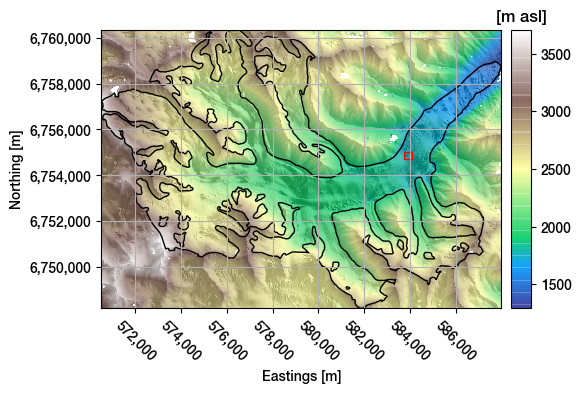
\includegraphics[scale=0.65]{../imgs/little Kluane glacier, post-surge/elevation.png}
\caption{Surface elevation of little Kluane glacier and surroundings with coverage of ice-penetrating radar measurements (red outline). Black outline from \citet{pfeffer2014randolph}}
\label{fig:lk_dem}
\end{subfigure}
\begin{subfigure}[c]{1\textwidth}
\centering
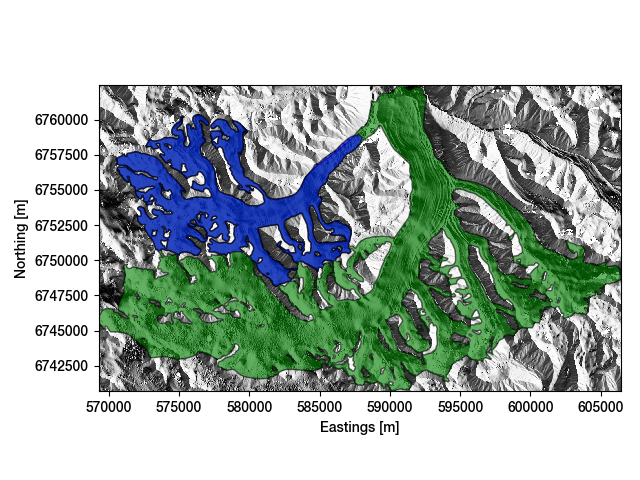
\includegraphics[scale=0.65]{../imgs/little Kluane glacier, post-surge/kluane_outlines.png}
\caption{Contours from \citet{pfeffer2014randolph} of little (blue) and big (green) Kluane glaciers.}
\label{fig:lk_outlines}
\end{subfigure}
\label{fig:lk_figs}
\caption{Elevation and location of the little Kluane glacier in the St. Elias mountains}
\end{figure}

The little Kluane glacier is the nickname given to a 20\,km long glacier covering $\sim$75\,km$^2$, part of the bigger Kluane glacier \fref{fig:lk_outlines}, located in the St. Elias moutains of Yukon. This glacier has been known to have surged from 2017 to 2018, showing an advance of 1.9 km \citep{main2019surge}. Master's student Andrew Nolan's research aims to understand the impact of climatic changes on surges dynamics.  

\FloatBarrier

\subsubsection{Data available}
The data available consists of two main different data sets with different time-scales which are before and during the end of the glacier's surge.
\\
The pre-surge data, from 2007, consists of a 20\,m resolution DEM from \citet{berthier2008spot5}, 240\,m resolution surface velocities from ITS\_LIVE \citeg{gardner2019its_live} and a glacier outline delimited by Andrew Nolan.
The post-surge data, from 2018 to 2019, consists of a 20\,m resolution DEM from (Need citation from Étienne, see july 10 email), 240\,m resolution surface velocites from ITS\_LIVE \citeg{gardner2019its_live} and a glacier outline also delimited by Andrew Nolan. 
\\

Also available is elevation change from 2007 to 2018, an 11 year time-scale. Ice thickness measurements from a GPR survey. Those measurements cover a very small area of the glacier \fref{fig:lk_dem} of around 0.03\,km$^2$.

\FloatBarrier

\section{The global consensus estimate: assessing the error}

\textbf{Some wonky inconsistencies with the 4-panels figures, need to figure out a consistent way to plot them}
\\
Following \textit{ITMIX}, \citet{farinotti2019consensus} bettered the earlier global estimate from \citeauthor{huss2012distributed} \citeyear{huss2012distributed}. Findings from \textit{ITMIX} were used to infer ice thickness of all the glaciers around the glob, using five different models and weighting each of their results to minimize the error. The computed models are \href{https://www.research-collection.ethz.ch/handle/20.500.11850/315707}{available online}. The increasing availability of globally produced datasets raises the need to acknowledge their quality as they are expected to be used in modelling specific glacier dynamics.
Real ice thickness measurements can help us better the approximation made by \citet{farinotti2019consensus}. First, we need to assess the model's error by comparing it to our point data.
%However, as the quality of the GPR data is limited and the time scales of the ice thickness models is unknown or very large \citep{farinotti2019consensus}, a precise quantification of the error is limited.
For $h'$ and $h$, the modelled and measured thickness values, we can compute the error 
\begin{equation}
\Delta h = h' - h
\label{eq:error}
\end{equation} by transforming our GPR point data to cell data, the format in which the model is computed. As there are more than one point by cell, the mean value of the point thickness data is taken for each grid cell according to the model's resolution. From equation \ref{eq:error}, positive values of $\Delta h$ imply \textit{overestimation} of ice thickness from the model and negative values imply \textit{underestimation}.

\subsection{North Glacier}
The modelled distributed ice thickness \fref{fig:ng_thickness} from \citet{farinotti2019consensus} for North Glacier seems to respect the measured data, however noting a general trend of overestimating, as seen on Figures \ref{fig:xy_ng_thickness} and \ref{fig:ng_consensus_error_zoomed}.

\begin{figure}[h!]
\centering
\makebox[\textwidth][c]
{
\begin{subfigure}{0.5\linewidth}
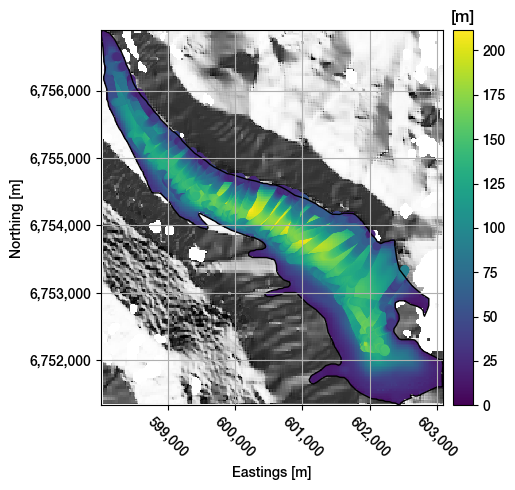
\includegraphics[width=5cm]{../imgs/North glacier/consensus_thickness.png}
\caption{The modelled ice thickness, glacier extent}
\label{fig:ng_thickness}
\end{subfigure}
\hfill
\begin{subfigure}{0.5\linewidth}
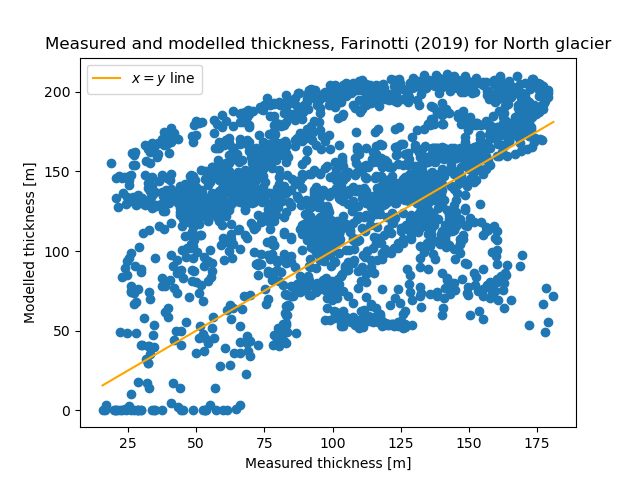
\includegraphics[width=5cm]{../imgs/North glacier/xy_scatter_consensus.png}
\caption{The grid-cell averaged measured data against modelled thickness data}
\label{fig:xy_ng_thickness}
\end{subfigure}
}
\makebox[\textwidth][c]{
\subcaptionbox{The modelled ice thickness, zoomed extent\label{fig:ng_consensus_thickness_zoomed}}[0.5\linewidth][c]{
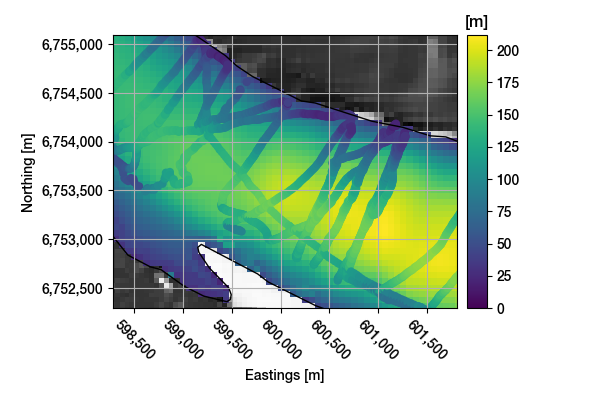
\includegraphics[width=7cm]{../imgs/North glacier/consensus_thickness_zoomed.png}}
\hfill
\subcaptionbox{The model's error, zoomed extent\label{fig:ng_consensus_error_zoomed}}[0.5\linewidth][c]{
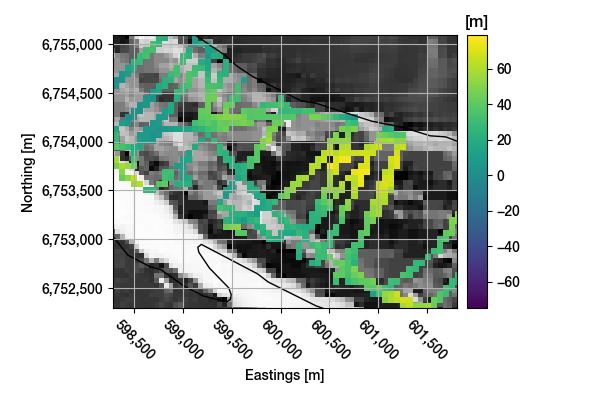
\includegraphics[width=7cm]{../imgs/North glacier/consensus_error_zoomed.png}}
}
\caption{Modelled thickness for North glacier \citep{farinotti2019consensus}. Points shown on Figures \ref{fig:ng_thickness} and \ref{fig:ng_consensus_thickness_zoomed} are thickness measurements from the GPR survey.}
\end{figure}
\FloatBarrier

\subsection{South Glacier}
The modelled distributed ice thickness \fref{fig:ng_thickness} from \citet{farinotti2019consensus} for South Glacier seems to respect the measured data, with no striking trend of either over or under estimating, as seen on Figures \ref{fig:xy_ng_thickness} and \ref{fig:ng_consensus_error_zoomed}.
\begin{figure}[h!]
\centering
\makebox[0.6\textwidth][c]
{
\begin{subfigure}{0.6\linewidth}
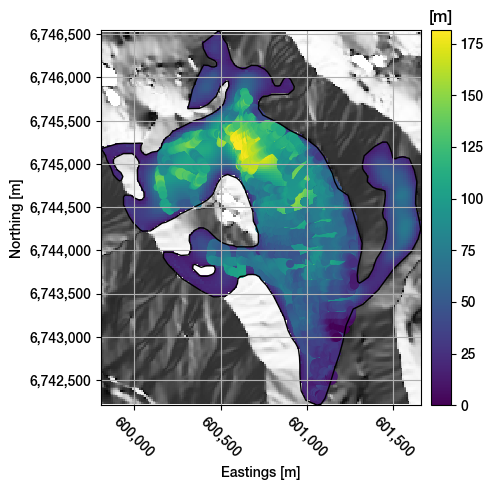
\includegraphics[width=0.8\textwidth]{../imgs/South glacier/consensus_thickness.png}
\caption{The modelled ice thickness, glacier extent}
\label{fig:sg_thickness}
\end{subfigure}
\hfill
\begin{subfigure}{0.6\linewidth}
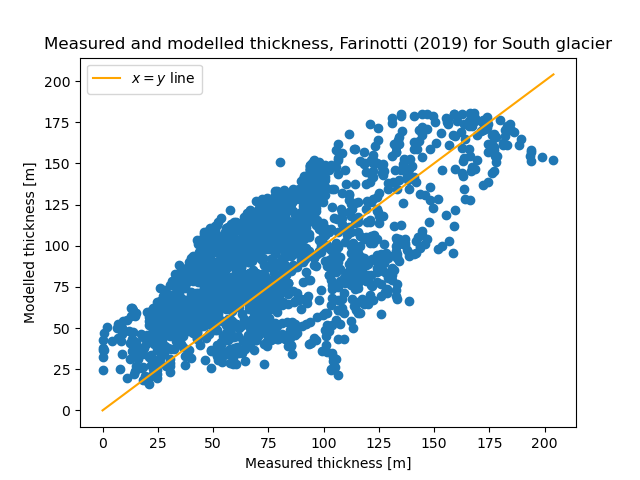
\includegraphics[width=0.8\textwidth]{../imgs/South glacier/xy_scatter_consensus.png}
\caption{The grid-cell averaged measured data against modelled thickness data}
\label{fig:xy_sg_thickness}
\end{subfigure}
}
\makebox[\textwidth][c]{
\subcaptionbox{The modelled ice thickness, zoomed extent\label{fig:sg_consensus_thickness_zoomed}}[0.6\textwidth][c]{
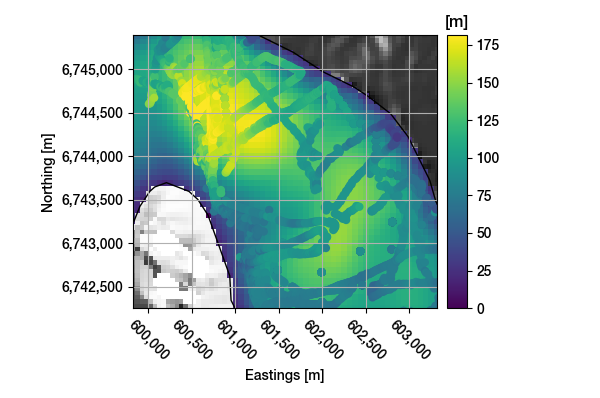
\includegraphics[width=\linewidth]{../imgs/South glacier/consensus_thickness_zoomed.png}}
\hfill
\subcaptionbox{The model's error, zoomed extent\label{fig:sg_consensus_error_zoomed}}[0.65\textwidth][c]{
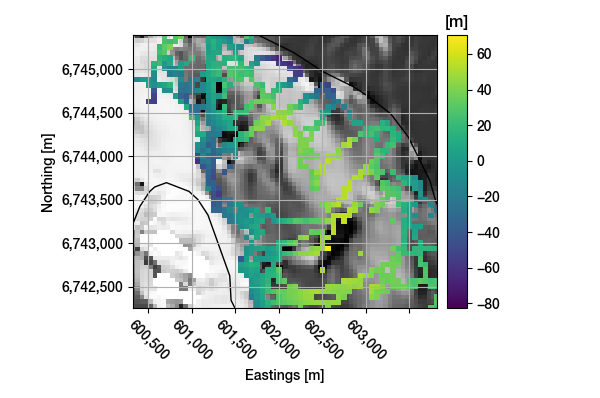
\includegraphics[width=\linewidth]{../imgs/South glacier/consensus_error_zoomed.png}}
}
\caption{Modelled thickness for South glacier \citep{farinotti2019consensus}. Points shown on \ref{fig:sg_thickness} and \ref{fig:sg_consensus_thickness_zoomed} are thickness measurements from the GPR survey.}
\end{figure}
\FloatBarrier

\subsection{Kaskawulsh Glacier}

The vast Kaskawulsh Glacier sees modelled ice thickness \citep{farinotti2019consensus} ranging from 0 to 800 meters \fref{fig:kaska_thickness}. The model correctly guesses the maximum thickness values but overestimates the thinner ice measurements (Figures \ref{fig:xy_kaska_thickness} and \ref{fig:kaska_consensus_error_zoomed}).

\begin{figure}[h!]
\centering
\makebox[\textwidth][c]
{
\begin{subfigure}{0.65\textwidth}
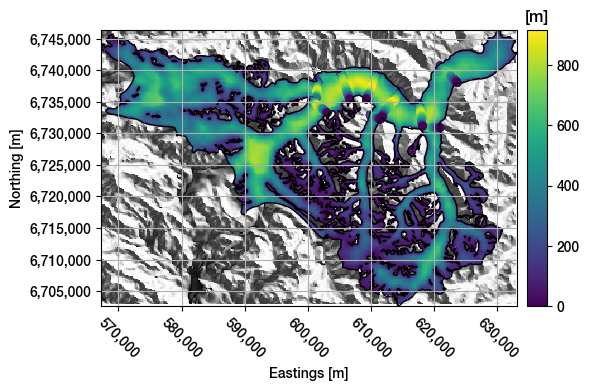
\includegraphics[width=\linewidth]{../imgs/Kaskawulsh glacier/consensus_thickness.png}
\caption{The modelled ice thickness, glacier extent}
\label{fig:kaska_thickness}
\end{subfigure}
\centering
\begin{subfigure}{0.65\textwidth}
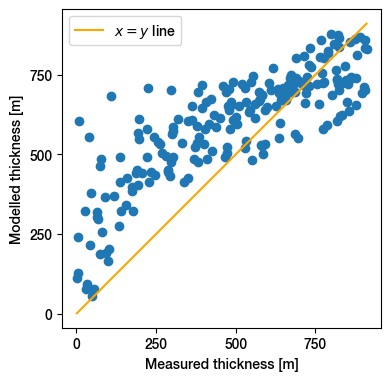
\includegraphics[width=0.8\textwidth]{../imgs/Kaskawulsh glacier/xy_scatter_consensus.png}
\caption{The grid-cell averaged measured data against modelled thickness data}
\label{fig:xy_kaska_thickness}
\end{subfigure}
}
\makebox[\textwidth][c]{
\subcaptionbox{The modelled ice thickness, zoomed extent\label{fig:kaska_consensus_thickness_zoomed}}[0.65\textwidth][c]{
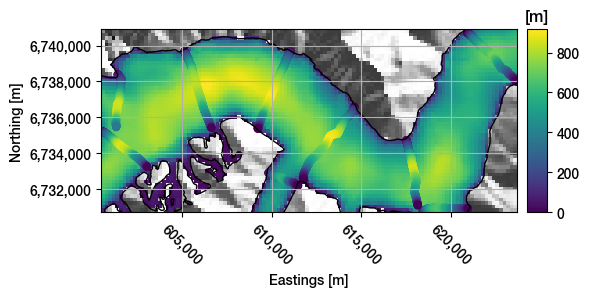
\includegraphics[width=\linewidth]{../imgs/Kaskawulsh glacier/consensus_cropped_thickness.png}}
\hfill
\subcaptionbox{The model's error, zoomed extent\label{fig:kaska_consensus_error_zoomed}}[0.65\textwidth][c]{
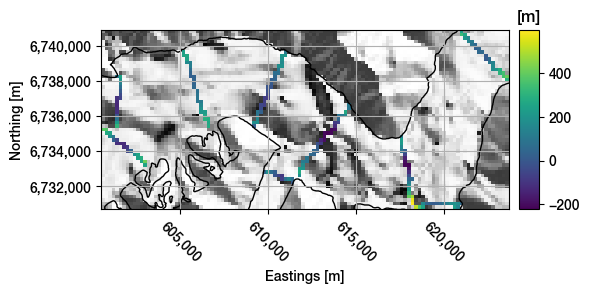
\includegraphics[width=\linewidth]{../imgs/Kaskawulsh glacier/consensus_cropped_error.png}}
}
\caption{Modelled thickness for South glacier \citep{farinotti2019consensus}. Points shown on \ref{fig:kaska_thickness} and \ref{fig:kaska_consensus_thickness_zoomed} are thickness measurements from the GPR survey.}
\end{figure}
\FloatBarrier

\subsection{Job Glacier}

\begin{figure}[h!]
\centering
\makebox[\textwidth][c]{
\begin{subfigure}{0.6\linewidth}
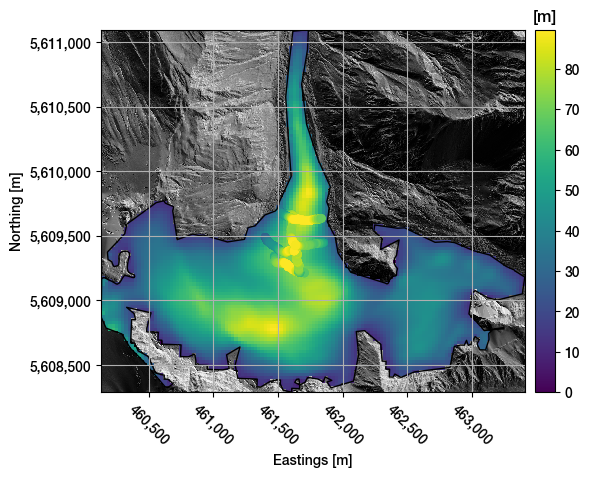
\includegraphics[width=8cm]{../imgs/Job glacier/consensus_thickness.png}
\caption{The modelled ice thickness, glacier extent}
\label{fig:job_thickness}
\end{subfigure}
\hfill
\begin{subfigure}{0.6\linewidth}
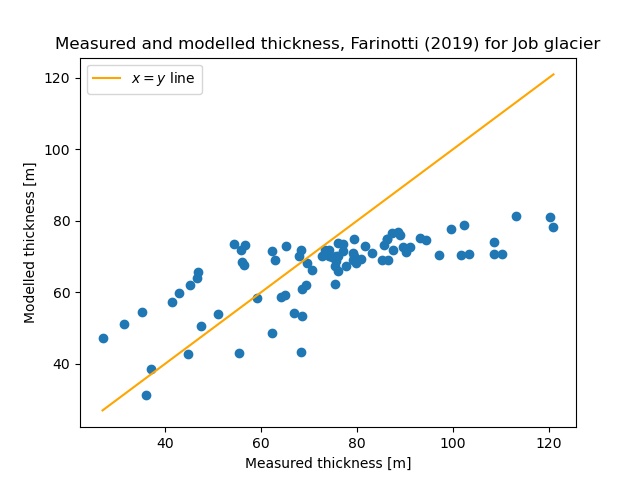
\includegraphics[width=7cm]{../imgs/Job glacier/xy_scatter_consensus.png}
\caption{The grid-cell averaged measured data against modelled thickness data}
\label{fig:xy_job_thickness}
\end{subfigure}
%
}
\makebox[\textwidth][c]{
\subcaptionbox{The modelled ice thickness, GPR coverage extent \label{fig:job_thickness_cropped}}[0.6\linewidth][c]{
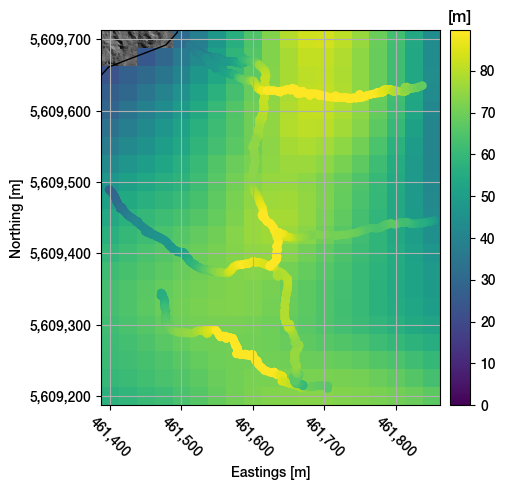
\includegraphics[width=8cm]{../imgs/Job glacier/consensus_cropped_thickness.png}}
\hfill
\subcaptionbox{The model's error, GPR coverage extent \label{fig:job_consensus_error}}[0.6\linewidth][c]{
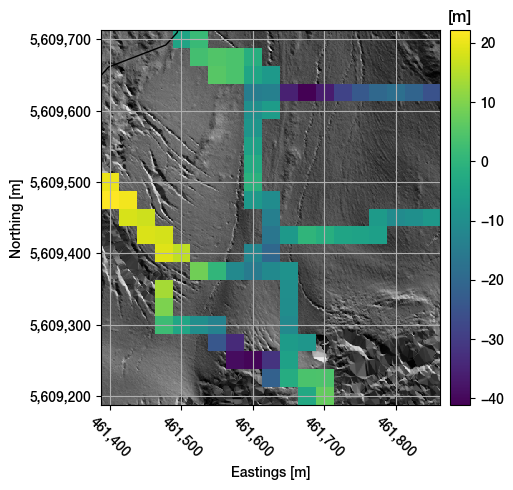
\includegraphics[width=8cm]{../imgs/Job glacier/consensus_cropped_error.png}}
}
\caption{Modelled thickness for Job glacier \citep{farinotti2019consensus}. Points shown on \ref{fig:job_thickness} and \ref{fig:job_thickness_cropped} are thickness measurements from the GPR survey.}

\end{figure}

The modelled distributed ice thickness \fref{fig:job_thickness} from \citet{farinotti2019consensus} puts the thinner ice upon the higher elevations and the thicker ice in the lower areas, all the way down the terminus of the glacier. Also shown on Figure \ref{fig:job_thickness} is the area covered by the GPR point data. A closer look of the model \fref{fig:job_thickness_cropped} can show us the discrepancies between the modelled and measured data. The larger errors are located upon the margins of the glaciers, modelling thicker and thinner ice to the western and eastern margin respectively \fref{fig:job_consensus_error}. The measured and modelled ice thickness is plotted on Figure \ref{fig:xy_job_thickness}. The higher errors from the models are for larger values of ice thickness, therefore underestimating the glacier's bed topography.
\FloatBarrier

\subsection{Little Kluane Glacier}
\begin{figure}[h!]
\makebox[\textwidth][c]{
\centering
\subcaptionbox{The modelled ice thickness, glacier extent\label{fig:lk_thickness}}[0.65\textwidth][c]{
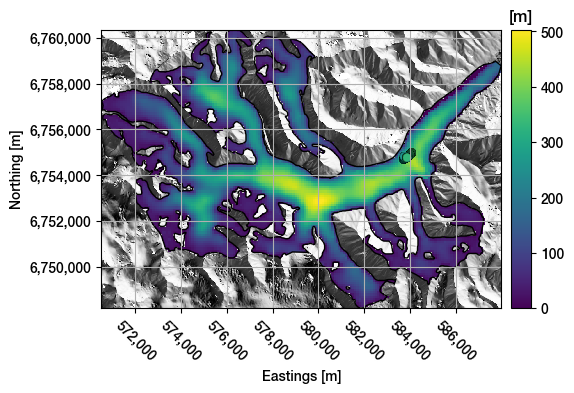
\includegraphics[width=\linewidth]{../imgs/little Kluane glacier, post-surge/consensus_thickness.png}}
\hfill
\subcaptionbox{The grid-cell averaged measured data against modelled thickness data\label{fig:xy_lk_thickness}}[0.65\textwidth][c]{
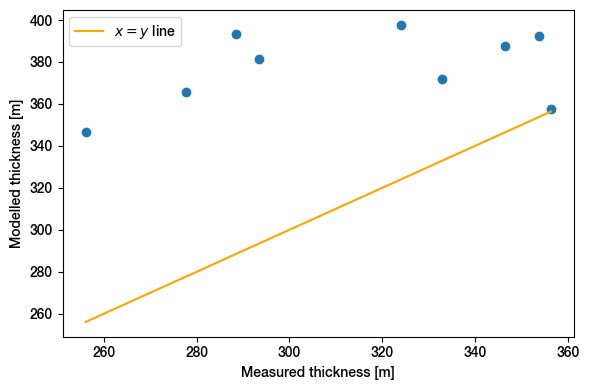
\includegraphics[width=\linewidth]{../imgs/little Kluane glacier, post-surge/xy_scatter_consensus.png}}
}
\makebox[\textwidth][c]{
\subcaptionbox{The modelled ice thickness, GPR coverage extent\label{fig:lk_thickness_cropped}}[0.65\textwidth][c]{
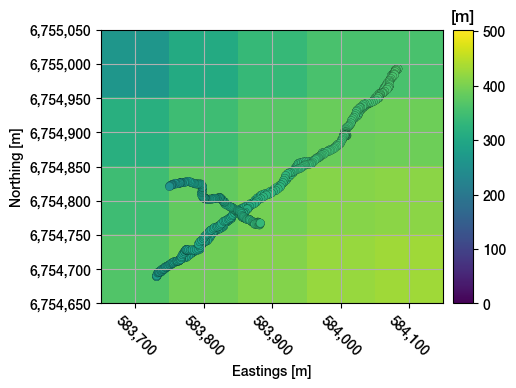
\includegraphics[width=\linewidth]{../imgs/little Kluane glacier, post-surge/consensus_cropped_thickness.png}}
\hfill
\subcaptionbox{The model's error, GPR coverage extent\label{fig:lk_consensus_error}}[0.65\textwidth][c]{
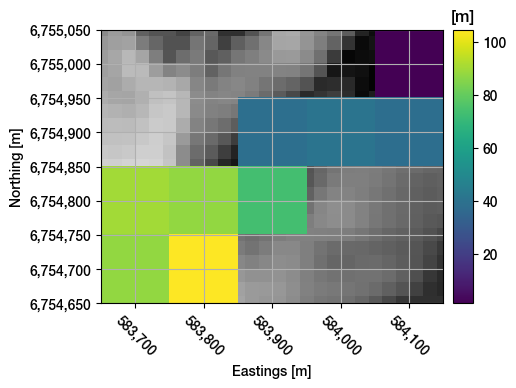
\includegraphics[width=\linewidth]{../imgs/little Kluane glacier, post-surge/consensus_cropped_error.png}}
}
\caption{Modelled thickness for little Kluane glacier \citep{farinotti2019consensus}. Points shown on \ref{fig:lk_thickness} and \ref{fig:lk_thickness_cropped} are thickness measurements from the GPR survey.}
\end{figure}


Little Kluane being a much bigger glacier than Job, the absolute thickness is much greater. The modelled distributed thickness puts the thicker ice in the lower areas. Because the data was acquired during the surge, covering a great section without having to cross crevasses is a difficult task, hence the smaller GPR coverage \fref{fig:lk_thickness_cropped}. The produced error-map \fref{fig:lk_consensus_error} has so few cells that its analysis gives little insight into the model's representation. However, it is showing errors of up to a 100\,m. The model is strictly overestimating the glacier's thickness \fref{fig:xy_lk_thickness}. The time-scales of the model produced by \citet{farinotti2019consensus} are not available (Farinotti, 2020, personal communication). However, we suspect that based on the timing of the work, the data used is pre-surge. The strict over-estimation of the model is then surprising; one would expect the ice to be thicker after surging, especially down-glacier, where the measurements are coming from.

\FloatBarrier
\pagebreak

\subsection{Error quantification}
By comparing the values from the model's cells and the cell averaged GPR data, we can compute the error $\Delta h$ according to equation \ref{eq:error}. It is always good to first look at the error histograms as they can tell us a lot about the general distribution:
% Load histograms %
\begin{figure}[h]
\centering
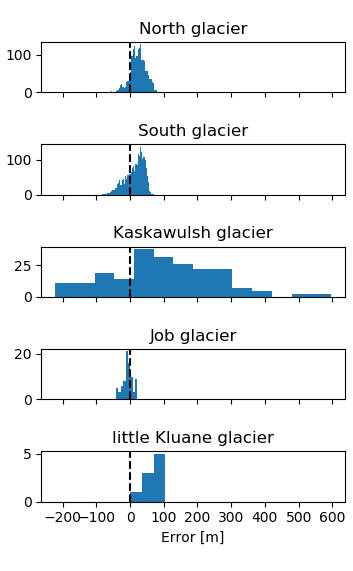
\includegraphics[width=0.5\linewidth]{../imgs/hists.png}
\caption{Error distribution from \citet{farinotti2019consensus} for the different test cases}
\label{fig:hists}
\end{figure}
\FloatBarrier
The histograms of North and South glacier are both slightly asymmetrical and showing a non-zero mode, hence generally overestimating the ice thickness. Those two cases have finer histograms from a much greater number of observed cells to compare data from. The Kaskawulsh Glacier's histogram is also asymmetrical and generally showing ice thickness overestimation. However, it is also showing much greater standard deviation, with errors ranging from -200\,m to 600\,m. This is probably due to the impressive scale difference from Kaskawulsh and other test cases. Job Glacier is the only case where the model from \citet{farinotti2019consensus} is generally underestimating the ice thickness, showing a mode slightly under zero. The Little Kluane Glacier is also showing non-zero mean and mode altough the very small number of cells make the histogram's analysis difficult.
\\
Different error metrics can be computed, such as the mean, the standard deviation, the median. Other interesting metrics are the mean absolute error $MAE$, defined as: 
\begin{equation}
MAE = \frac{1}{n}\sum_{i=0}^{n}|\Delta h_i|
\end{equation}
where n is the number of cell averaged ice thickness measurements. The $MAE$ tells us about the absolute deviation from zero, giving us an idea of the scale of the general error, omitting the sign. Also interesting to compute is the root mean square error $RMSE$:
\begin{equation}
RMSE = \sqrt{\frac{1}{n}\sum_{i=0}^{n}(\Delta h_i)^2}
\end{equation}
In $RMSE$'s case, the higher error values have more weight, resulting in a greater $RMSE$. The different error metrics are shown on Table \ref{tab:error_table}. 

% Load data from the error csv %
\DTLloaddb{errdata}{../imgs/stats-abs.csv}
\begin{table}[h!]
\centering
\small
\caption{Error from the ice thickness models computed by \citet{farinotti2019consensus} for the glacier test cases against cell averaged GPR measurements. Note that every metric is shown in metres.}
\label{tab:error_table}
\noindent\makebox[\textwidth]{
\begin{tabular}{|c|c|c|c|c|c|c|c|}
\hline
% Header %
\textbf{Glacier} & \textbf{Mean} & \textbf{Std} & \textbf{Median} & \textbf{Max} & \textbf{Min} & $\boldsymbol{MAE}$ & $\boldsymbol{RMSE}$
% Iterated csv data %
\DTLforeach{errdata}{\glacier=Glacier,\mean=Mean,\std=Std,\med=Median,\max=Maximum, \min=Minimum, \abs=Mean absolute,\mse=RMSE}
{\\ \hline \glacier & \mean & \std & \med & \max & \min & \abs & \mse}
\\ \hline
\end{tabular}
}
\end{table}
\FloatBarrier
The different error metrics seems to be correlated with the scale of the glacier, with smaller errors from Job Glacier, to North and South Glaciers, Little Kluane and finally Kaskawulsh glacier. It is then difficult to compare the different computed error metrics and really capture any general trend. However, Table \ref{tab:error_table}'s data can confirm that the only generally underestimated ice thickness is in Job Glacier's case. To take care of the different scales, we can take a loot at the relative error:
\begin{equation}
\delta h = \frac{\Delta h}{h}
\end{equation}
This error however is problematic for very small or null values of $h$, lending to unreasonably large or non numeric mean values. However, we can still try to compute the same metrics and see what they look like (Table \ref{tab:rel_error_table}).

% Load data from the error csv %
\DTLloaddb{relerrdata}{../imgs/stats-rel2.csv}
\begin{table}[h!]
\centering
\small
\caption{Relative error from the ice thickness models computed by \citet{farinotti2019consensus} for the glacier test cases against cell averaged GPR measurements. Note that every metric is shown in percentages.}
\label{tab:rel_error_table}
\noindent\makebox[\textwidth]{
\begin{tabular}{|c|c|c|c|c|c|c|c|}
\hline
% Header %
\textbf{Glacier} & \textbf{Mean} & \textbf{Std} & \textbf{Median} & \textbf{Max} & \textbf{Min} & $\boldsymbol{MAE}$ & $\boldsymbol{RMSE}$
% Iterated csv data %
\DTLforeach{relerrdata}{\glacier=Glacier,\mean=Mean,\std=Std,\med=Median,\max=Maximum, \min=Minimum, \abs=Mean absolute,\mse=RMSE}
{\\ \hline \glacier & \mean & \std & \med & \max & \min & \abs & \mse}
\\ \hline
\end{tabular}
}
\end{table}

South and Kaskawulsh's glaciers error metrics are either non numeric or still disproportionate. We can avoid this problem by omitting smaller thickness values, setting an arbitrary acceptance threshold. By only comparing the relative error for $h >= 5$\,m, we get this table:

% Load data from the error csv %
\DTLloaddb{5relerrdata}{../imgs/stats-rel.csv}
\begin{table}[h!]
\centering
\small
\caption{Relative error from the ice thickness models computed by \citet{farinotti2019consensus} for the glacier test cases against cell averaged GPR measurements. Note that every metric is shown in percentages. Every value of $h < 5$\,m was omitted.}
\label{tab:5rel_error_table}
\noindent\makebox[\textwidth]{
\begin{tabular}{|c|c|c|c|c|c|c|c|}
\hline
% Header %
\textbf{Glacier} & \textbf{Mean} & \textbf{Std} & \textbf{Median} & \textbf{Max} & \textbf{Min} & $\boldsymbol{MAE}$ & $\boldsymbol{RMSE}$
% Iterated csv data %
\DTLforeach{5relerrdata}{\glacier=Glacier,\mean=Mean,\std=Std,\med=Median,\max=Maximum, \min=Minimum, \abs=Mean absolute,\mse=RMSE}
{\\ \hline \glacier & \mean & \std & \med & \max & \min & \abs & \mse}
\\ \hline
\end{tabular}
}
\end{table}

The relative error for South Glacier now looks more like North Glacier, which is to be expected, as they have both similar geographical localisations and GPR coverage. However, Kaskawulsh Glacier's relative error is lower, but not to more acceptable levels. With a mean absolute relative error of 112.76\,\%, the estimate from \citet{farinotti2019consensus} is on average either twice or half the measured value. Job Glacier and Little Kluane glaciers show a good fit with the observed data, with a mean relative error of -3.58\,\% and 21.22\,\%. However, the differences between the GPR coverage for every glacier is important (see Table \ref{tab:relgpr})

\DTLloaddb{relgpr}{../imgs/rel.csv}
\begin{table}[h!]
\centering
\small
\caption{Relative GPR coverage for the different glaciers. The relative coverage is the coverage area (Figure \ref{fig:ashape}) divided by the glacier's area from \citet{pfeffer2014randolph}.}
\label{tab:relgpr}
\noindent\makebox[\textwidth]{
\begin{tabular}{|c|c|}
\hline
% Header %
\textbf{Glacier} & \textbf{Relative GPR coverage\,[\%]}
% Iterated csv data %
\DTLforeach{relgpr}{\glacier=glac,\rel=rel}
{\\ \hline \glacier & \rel}
\\ \hline
\end{tabular}
}
\end{table}

\begin{figure}
\centering
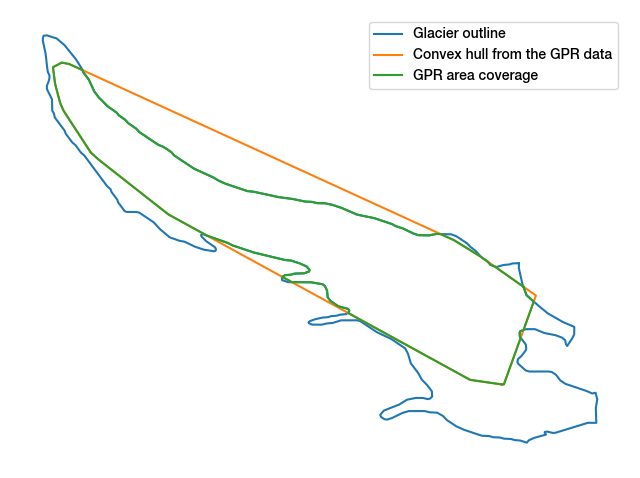
\includegraphics[width=0.7\textwidth]{../imgs/ashape.png}
\label{fig:ashape}
\caption{The intersection of the glacier's outline and the convex hull formed by the GPR points is the GPR coverage area. Showcased here is North Glacier's.}
\end{figure}

In North and South glacier's cases, the error analysis is probably telling us valid information about the mode as the GPR coverage is over 50\,\%. It is not clear, however, for Kaskawulsh Glacier: even if the computed relative coverage is of 12.14\,\%, the actual coverage is probably smaller given the geometry of the transects \fref{fig:kaska_consensus_thickness_zoomed}. The computed error metrics are nonetheless not convincing of a good fit. For Job and Little Kluane glaciers, the error analysis is not sufficient to tell if the model computed by \citet{farinotti2019consensus} is good or not given the poor GPR coverage of less than 5\,\% for both glaciers. Furthermore, the comparison of the model for little Kluane glacier is not coherent given that the ice thickness model was computed using pre-surge data for a much bigger glacier \fref{fig:lk_outlines} and that the GPR measurements were taken during the surge. 
\\
It is then particularly important for the multiple reasons above to at least try to better the available bed models from \citet{farinotti2019conensus} or even infer the bed topography from data in which we are confident in the time-scales.
\FloatBarrier

\section{GlaTe model}
\subsection{The full GlaTe algorithm}
The freely available online GlaTe model \citeg{langhammer2019glacier} aims to, using surface elevation, a glacier outline and ice thickness measurements, minimize the discrepancy between modelled and observed data.
\\
The GlaTe model initially estimates the distributed ice thickness $\hat{h}^{glac}$ using a physical model inspired by \citet{clarke2013ice}. This physical model takes as input a DEM and a glacier outline. With this available ice thickness data $h^{GPR}$, the algorithm reduces the observable error on this approximation by scaling the physical model $\hat{h}^{glac}$ by a coefficient $\alpha_{GPR}$ from  minimizing a cost function $q$ defined as
\begin{equation}
q = ||h^{GPR} - \alpha_{GPR}\hat{h}^{glac}||^2
\label{eq:cost_function}
\end{equation}
which is equivalent of a linear regression with a fixed (and null) intercept. This coefficient is used such that
\begin{equation}
h^{glac} = \alpha_{GPR}\hat{h}^{glac}
\label{eq:hglac}
\end{equation}
is a supposedly better overall approximation, giving a bigger weight to the observed data and minimizing the impact of generalized trends in the physical model.
Using this better approximation $h^{glac}$, the algorithm aims to solve this system of equations:
\begin{equation}
\begin{bmatrix} \lambda_1 \textrm{\textbf{G}}\\ \lambda_2 \textrm{\textbf{L}}\\ \lambda_3 \textrm{\textbf{B}}\\ \lambda_4 \textrm{\textbf{S}}\\ \end{bmatrix}
h^{est} = 
\begin{bmatrix} \lambda_1 h^{GPR}\\ \lambda_2 \nabla h^{glac} \\ 0 \\ 0 \end{bmatrix}
\end{equation}
where :
\begin{itemize}
\item $h^{est}$ is the modelled ice thickness distribution
\item $\lambda_1 \textrm{\textbf{G}}$ are used to fit the observed data within uncertainty
\item $\lambda_2 \textrm{\textbf{L}}$ are used to avoid systematic differences between observed and modelled data
\item $\lambda_3 \textrm{\textbf{B}}$ are used to ensure zero thickness at the boundaries
\item $\lambda_4 \textrm{\textbf{S}}$ are used to obtain a smoother surface, as \textbf{S} is a smoothing matrix.
\end{itemize}
The scalar values $\lambda_i$ are respective weights for every equation in the system and are tuned during the algorithm's run until an arbitrary error threshold for $h^{est}$ is met. The GlaTe model could be described as a physical method of ice thickness interpolation. The algorithm thus outputs three distributed ice thickness maps:
\begin{itemize}
\item The physical model $\hat{h}^{glac}$
\item The \textit{corrected} or rather scaled physical model $h^{glac} = \alpha_{GPR}\hat{h}^{glac}$
\item The final estimation $h^{est}$
\end{itemize}
Those can be observed for the test cases \fref{fig:glate_thickness} where the GlaTe algorithm was applied. The resulting modelled ice thickness $h^{est}$ shows a very small observable error \fref{fig:glate_xy}. 

\begin{landscape}
\begin{figure}[h!]
\makebox[1.5\textwidth][c]{
\centering
\begin{subfigure}{0.225\linewidth}
\centering
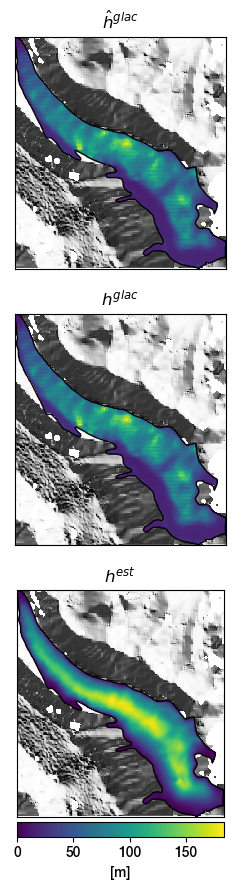
\includegraphics[height=4.5in]{../imgs/North glacier/glate_thickness_all_models.png}
\caption{North Glacier}
\label{fig:glate_ng_thickness}
\end{subfigure}
\hfill
\begin{subfigure}{0.225\linewidth}
\centering
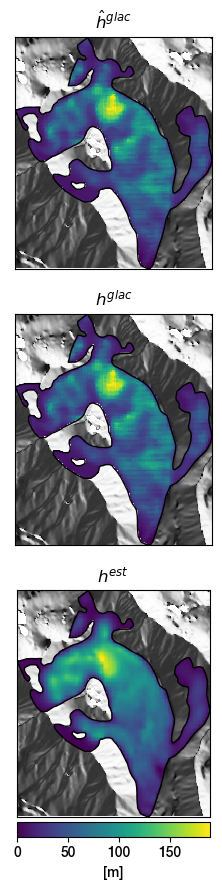
\includegraphics[height=4.5in]{../imgs/South glacier/glate_thickness_all_models.png}
\caption{South Glacier}
\label{fig:glate_sg_thickness}
\end{subfigure}
\hfill
\begin{subfigure}{0.225\linewidth}
\centering
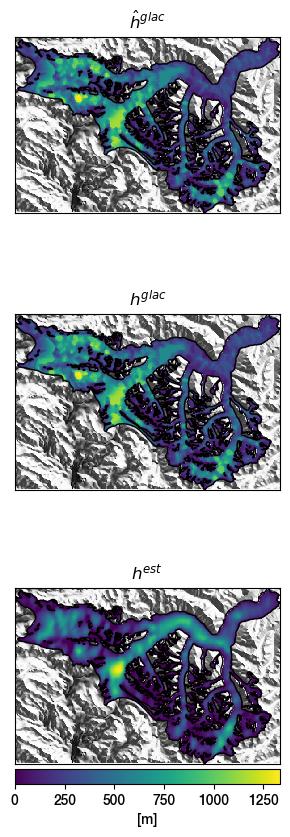
\includegraphics[height=4.5in]{../imgs/Kaskawulsh glacier/glate_thickness_all_models.png}
\caption{Kaskawulsh glacier}
\label{fig:glate_kaska_thickness}
\end{subfigure}
\hfill
\begin{subfigure}{0.225\linewidth}
\centering
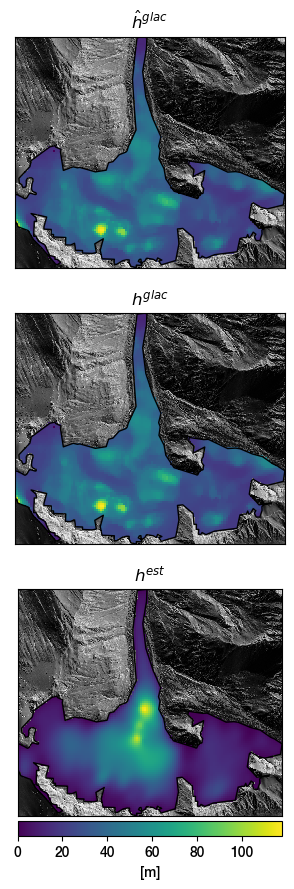
\includegraphics[height=4.5in]{../imgs/Job glacier/glate_thickness_all_models.png}
\caption{Job glacier}
\label{fig:glate_job_thickness}
\end{subfigure}
\hfill
\begin{subfigure}{0.225\linewidth}
\centering
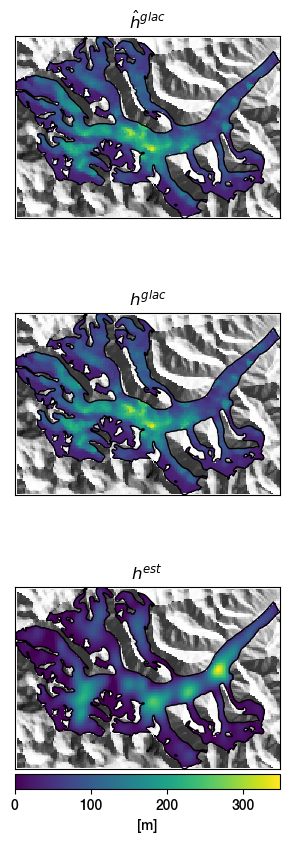
\includegraphics[height=4.5in]{../imgs/little Kluane glacier/glate_thickness_all_models.png}
\caption{Little Kluane glacier}
\label{fig:glate_lk_thickness}
\end{subfigure}
}
\caption{Thickness maps produced with the complete GlaTe algorithm for the test cases. Physical model is inspired from \citet{clarke2013ice}.}
\label{fig:glate_thickness}
\end{figure}
\end{landscape}
\FloatBarrier


\begin{figure}[h!]
\centering
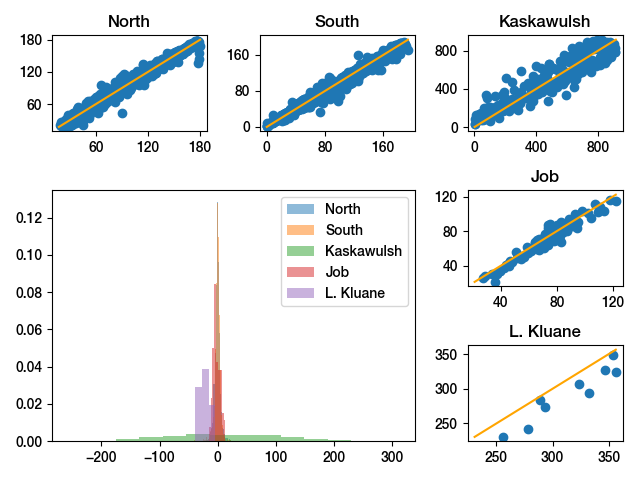
\includegraphics[width=0.75\textwidth]{../imgs/fiveplot_glate_full.png}
\caption{Scatterplot of the measured ($x$-axis) and modelled $h^{est}$ ($y$-axis) for the test cases. Bottom left are the normalised $h^{est}$ error [m] histograms of the different test cases. Physical model inspired by \citet{clarke2013ice}.}
\label{fig:glate_xy}
\end{figure}

Figure \ref{fig:glate_xy} gives the impression that the $h^{est}$ model is close to a perfect estimate of the bed ice thickness. However, this is due to the nature of the GlaTe algorithm, reducing the error for known data points only. We cannot assess the validity of a model from observing the error for known data points only, an educated, arbitrary opinion is necessary. When looking at the ice thickness fields produced by the complete GlaTe algorithm for the poorer coverage glaciers (Kaskawulsh, Job and Little Kluane), the thickness maps make little sense:
\begin{itemize}
\item Kaskawulsh Glacier's maximum ice thickness (1250\,m!) region is located in the upper part of the elevation range
\item Job Glacier shows very thin ice almost everywhere
\item Little Kluane Glacier shows thick ice at every tributary junction, diminishing in thickness in between
\end{itemize}

Due to nature of the GlaTe algorithm, there is little physical meaning in the resulting ice thickness field $h^{est}$. By itself, the GlaTe algorithm uses a physical model $\hat{h}^{glac}$ inspired by \citet{clarke2013ice}. By inputting another physical model $\hat{h}^{glac}$ for the rest of the algorithm, perhaps the resulting estimate $h^{est}$ will be better (Figure \ref{fig:fglate_thickness})? Once again, the resulting observable error from $h^{est}$ is very good (Figure \ref{fig:fglate_xy}). The error shows a very small standard deviation and is centred around zero for most of the cases. However, a few things can tell us that the resulting $h^{est}$ model is not exactly right:
\begin{itemize}
\item The resulting plot from using the physical model $\hat{h}^{glac}$ from \citet{farinotti2019consensus} (Figure \ref{fig:fglate_xy}) is quasi identical to the one produced using the complete GlaTe algorithm and it's physical model from \citet{clarke2013ice} (Figure \ref{fig:glate_xy}). This tells us that $h^{est}$ gives little meaning to the initial physical model for the cells with GPR coverage, resulting in the same data.
\item Kaskawulsh, Job and Little Kluane distributed ice thickness fields show very thin ice over almost all of the glaciers.
\end{itemize}

\begin{figure}[h!]
\centering
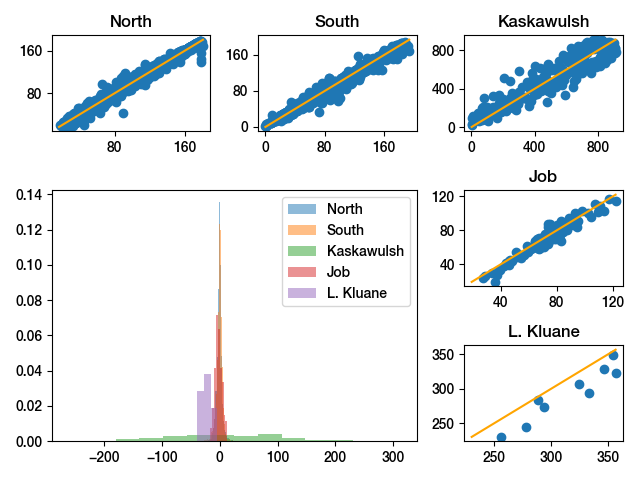
\includegraphics[width=0.75\textwidth]{../imgs/fiveplot_glate_farinotti_full.png}
\caption{Scatterplot of the measured ($x$-axis) and modelled $h^{est}$ ($y$-axis) for the test cases. Bottom left are the normalised $h^{est}$ error [m] histograms of the different test cases. Physical model from \citet{farinotti2019consensus}}
\label{fig:fglate_xy}
\end{figure}

\begin{landscape}
\begin{figure}[h!]
\makebox[1.5\textwidth][c]{
\centering
\begin{subfigure}{0.225\linewidth}
\centering
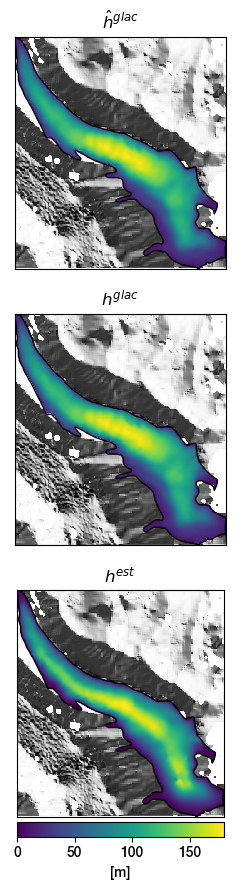
\includegraphics[height=4.5in]{../imgs/North glacier/farinotti_glate_thickness_all_models.png}
\caption{North Glacier}
\label{fig:fglate_ng_thickness}
\end{subfigure}
\hfill
\begin{subfigure}{0.225\linewidth}
\centering
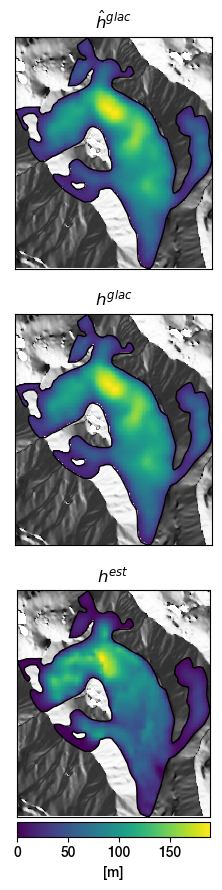
\includegraphics[height=4.5in]{../imgs/South glacier/farinotti_glate_thickness_all_models.png}
\caption{South Glacier}
\label{fig:fglate_sg_thickness}
\end{subfigure}
\hfill
\begin{subfigure}{0.225\linewidth}
\centering
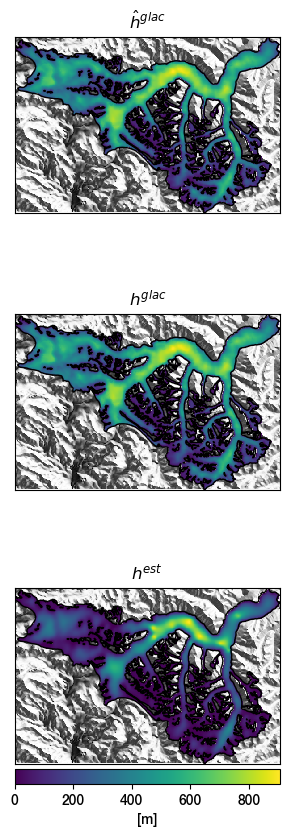
\includegraphics[height=4.5in]{../imgs/Kaskawulsh glacier/farinotti_glate_thickness_all_models.png}
\caption{Kaskawulsh glacier}
\label{fig:fglate_kaska_thickness}
\end{subfigure}
\hfill
\begin{subfigure}{0.225\linewidth}
\centering
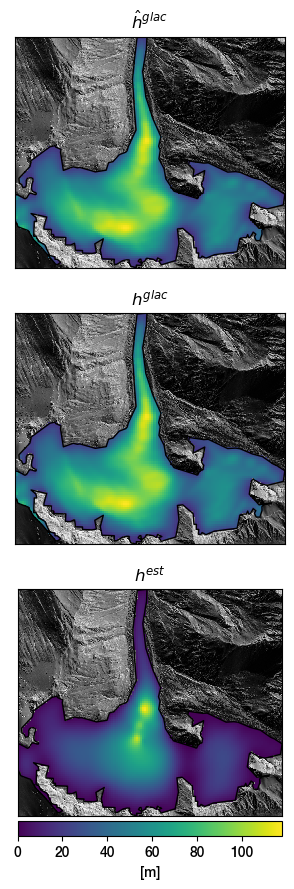
\includegraphics[height=4.5in]{../imgs/Job glacier/farinotti_glate_thickness_all_models.png}
\caption{Job glacier}
\label{fig:fglate_job_thickness}
\end{subfigure}
\hfill
\begin{subfigure}{0.225\linewidth}
\centering
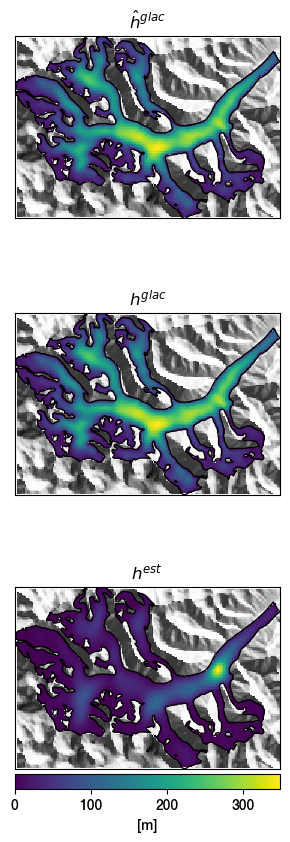
\includegraphics[height=4.5in]{../imgs/little Kluane glacier/farinotti_glate_thickness_all_models.png}
\caption{Little Kluane glacier}
\label{fig:fglate_lk_thickness}
\end{subfigure}
}
\caption{Thickness maps produced with the GlaTe algorithm and $\hat{h}^{glac}$ from \citet{farinotti2019consensus} for the test cases.}
\label{fig:fglate_thickness}
\end{figure}
\end{landscape}
\FloatBarrier
It seems like the GlaTe algorithm does a poor job of modelling distributed ice thickness when the GPR coverage is not all over the glacier. To verify the full GlaTe algorithm's performance over glaciers with worse GPR coverage, a small sample of points on North Glacier was arbitrarily selected and the resulting GPR data was set as input $h^{GPR}$ trough the GlaTe algorithm. The resulting model (Figure \ref{fig:ng_fewpoints_thickness}) was compared against the complete data set . $h^{est}$ ended up, like in the precedent cases, severely underestimating the ice thickness. The scatterplot (Figure \ref{fig:ng_fewpoints_xy}) shows that $h^{est}$ only fits the input data, ignoring the rest of the glacier. The entire GlaTe algorithm is then not a good approach to obtain bed topography for our test cases.
\begin{figure}[h!]
\centering
\makebox[\textwidth][c]{
\begin{subfigure}{0.6\linewidth}
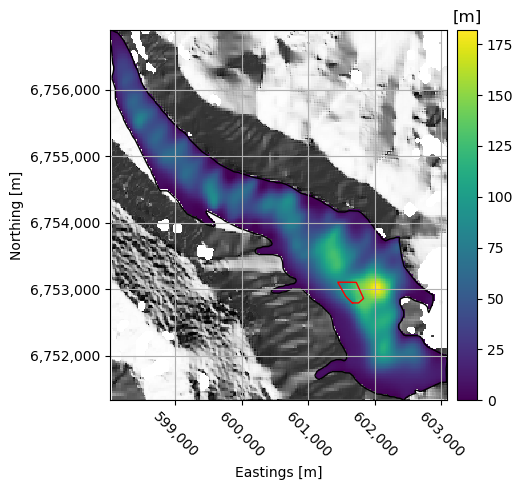
\includegraphics[width=\linewidth]{../imgs/North glacier, fewpoints/fewpoints_glate_farinotti_full_thickness_ashape.png}
\caption{The modelled ice thickness $h^{est}$ with physical model $\hat{h}^{glac}$ from \citet{farinotti2019consensus} as input. Red outline is the the GPR coverage area set as input data for the GlaTe algorithm.}
\label{fig:ng_fewpoints_thickness}
\end{subfigure}
\hfill
\begin{subfigure}{0.6\linewidth}
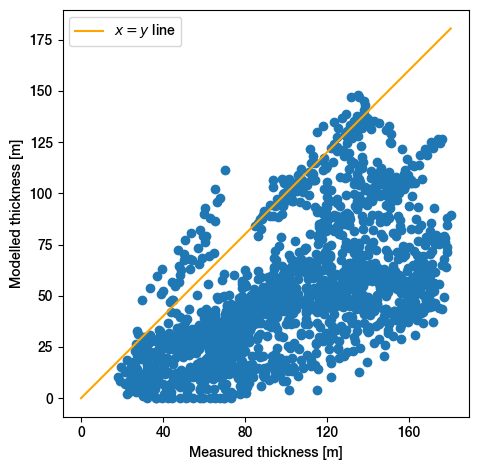
\includegraphics[width=\linewidth]{../imgs/North glacier/xy_scatter_fewpoints_glate_farinotti_full.png}
\caption{The measured against modelled thickness}
\label{fig:ng_fewpoints_xy}
\end{subfigure}
}
\caption{Testing the GlaTe algorithm for North Glacier with only a few GPR points as input data.}
\end{figure}
\FloatBarrier

\subsection{Verifying $\alpha_{GPR}$}
An interesting approach from the GlaTe algorithm is to scale an ice thickness model $\hat{h}^{glac}$ by a scalar $\alpha_{GPR}$. This scalar, obtained by minimizing the cost function from equation \ref{eq:cost_function}, is then used to obtain a \textit{better} approximation following equation \ref{eq:hglac}. To compute this scalar\footnote{Or simply \href{https://github.com/aleximorin}{use the pyGM library available on GitHub!} More information in the appendix.}, one needs to:
\begin{enumerate}
\item Transform the GPR point data to cell data. This is $h^{GPR}$. This raster needs to be of the same resolution and size as the ice thickness model $\hat{h}^{glac}$. 
\item Compute the coefficient $\alpha_{GPR}$ by minimising the cost function from equation \ref{eq:cost_function}. This can be done using your favorite least square method.
\item Multiply the initial $\hat{h}^{glac}$ by the $\alpha_{GPR}$ value obtained at step 2 to obtain $h^{glac}$.
\end{enumerate}
However, this approach should only better our estimation if a good coverage of the radar data is had, which is not the case for our study sites of Job and little Kluane. We can use our test cases with a better coverage, North and South glacier, to check if the values for $\alpha_{GPR}$ we obtain for an arbitrary number of GPR points resemble the \textit{best} value by considering it to be the one we obtain with our complete GPR data set. By randomly selecting an arbitrary number $N$ of GPR data points, their corresponding modelled cells and computing the equivalent $\alpha_{GPR}$ multiple (many many much) times, we can estimate the distribution of $\alpha_{GPR}$ for $N$ data points\footnote{The \href{https://github.com/aleximorin/USRA-2020-AlexiMorin/blob/master/compare_alpha.py}{code} used for this sampling is available on GitHub}.
\begin{figure}[h!]
\subfloat[North glacier]{\label{fig:ng_alpha_dist}\includegraphics[scale=0.5]{../alpha_compare/alpha_joyplot_North glacier_0.png}}
\\
\subfloat[South glacier]{\label{fig:sg_alpha_dist}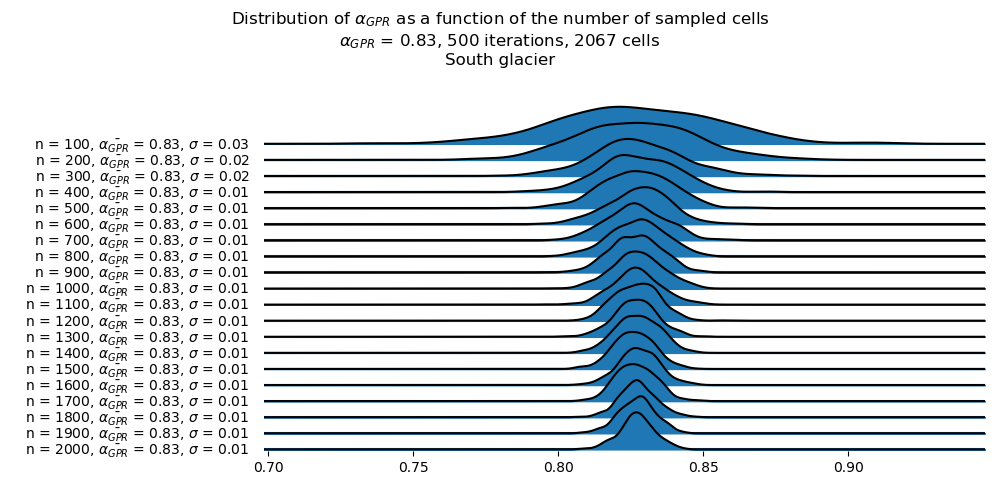
\includegraphics[scale=0.5]{../alpha_compare/alpha_joyplot_South glacier_0.png}}
\caption{Distribution of $\alpha_{GPR}$ for randomly sampled N cells}
\label{fig:alpha_dist}
\end{figure}
We see that distribution is strongly centered on the \textit{true} value of $\alpha_{GPR}$ and showing a rather small standard deviation for both cases \fref{fig:alpha_dist}. 
\\
\\
However, to represent the true spatial distribution of our datasets, we need to sample such random data. By randomly selecting one GPR data point and only the nearest cells, we can approximate such a random \textit{clumped} distribution for a more credible case. The distribution is less strongly centred on the \textit{true} value of $\alpha_{GPR}$ for small values of $N$ and shows a much greater standard deviation \fref{fig:alpha_dist_block}. The distribution is also strongly bimodal for increasing values of $N$. This is likely due to the less extreme nature of the models, underestimating and overestimating ice thickness in the lower and higher regions.
\\
\begin{figure}[h!]
\subfloat[North glacier]{\label{fig:ng_alpha_dist}\includegraphics[scale=0.5]{../alpha_compare/alpha_joyplot_North glacier_2.png}}
\\
\subfloat[South glacier]{\label{fig:sg_alpha_dist}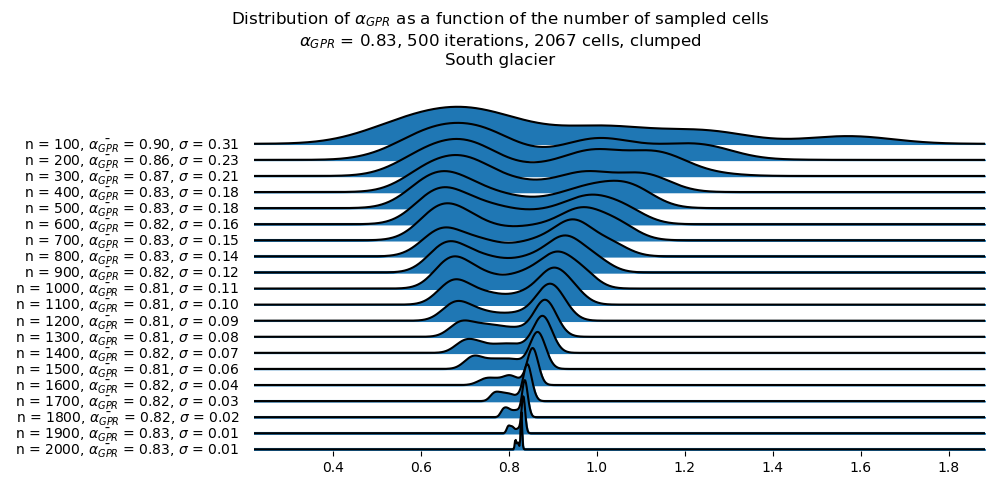
\includegraphics[scale=0.5]{../alpha_compare/alpha_joyplot_South glacier_2.png}} 
\caption{Distribution of $\alpha_{GPR}$ for randomly sampled N clumped cells}
\label{fig:alpha_dist_block}
\end{figure}
\\
For an ice thickness estimate $h^{glac}$ in which one is confident, such as the model from \citet{farinotti2019consensus}, one can scale it by a factor of $\alpha_{GPR}$ computed from equations \ref{eq:cost_function} and \ref{eq:hglac}. This model should be a \textit{better} model following Figure \ref{fig:alpha_dist_block}.
\FloatBarrier
\section{Appendix}
\subsection{pyGM: Tool for comparing glacier models}
I plan to fill this section up when I have the time to do further polishing following Andrew's suggestions. I'd like this section to be a guide on what this library can do.
\subsection{The Kaskawulsh glacier}
As part of Young et al. (references needed) article about the Kaskawulsh glacier's mass balance, flux gates area were computed. To compute those flux gates, one needs bed topography data, coming from either real world measurements or from inference. Ground penetrating radar data for this particular glacier was collected in the summers of 2018 and 2019. Flux gate area was computed by past undergraduate student Rebecca Latto in the summer of 2019 by summing the ice thickness values multiplied by 10, thus assuming a constant 10 meters distance between the point data.
\\
\\
As part of this ice thickness inference project, the differences between modelled and measured data for the Kaskawulsh glacier was computed. The main goal was to evaluate the potential error that would be made for the flux gate's area if one was to use modelled thickness data.
Latto's data was unfortunately not geo-referenced: for a given line, the only information had was that the points were along the line and separated by a constant distance of 10 meters. However, splitting the lines in such a way, using QGIS, did not work as the algorithm ended up outputting more or less points than that of Latto's data. Therefore a 1 to 1 connection could not be established.
\\
\\
What was done was that a given line was split up in as many points as there was thickness data for it. The distances between the points were then computed, resembling more or less 10 meters\footnote{The \href{https://github.com/aleximorin/USRA-2020-AlexiMorin/blob/master/treat_kaskawulsh_files.py}{code} used for this task and the \href{https://github.com/aleximorin/USRA-2020-AlexiMorin/blob/master/kaska_gps.csv}{data} produced is available on GitHub}.Having the $(x, y)$ coordinates meant that it could then be used to compare the measured thickness with models by extracting model values at those $(x, y)$ coordinates (Figures \ref{fig:kaska_consensus_thickness_zoomed} and \ref{fig:xy_kaska_thickness}).
\\
\\
To note is that some problems were had noting the orientation of the data. It was assumed that the transects data was orientated down glacier. This can be a problem when computing the error as the differences between the modelled and the observed data. However, it should not be a major problem when computing the differences between the modelled and measured area of the transects.

To compute the modelled flux gate areas, modelled ice thickness values $\hat{h}$ were extracted at every $(x, y)$ point were there was measured data. The distances between the points were computed as
\begin{equation}
d=\sqrt{(x_i - x_{i-1})^2 + (y_i - y_{i-1})^2}
\end{equation}
and the area was computed using numpy's trapezoid integration (need reference?) algorithm. The \href{https://github.com/aleximorin/USRA-2020-AlexiMorin/blob/master/transects_area_GATE_v2.csv}{data} generated is available on GitHub and visible on Table \ref{tab:area}.

\DTLloaddb{areadb}{../imgs/transects-area.csv}
\begin{table}[h!]
\centering
\caption{Gate areas computed from GPR data, \citet{farinotti2019consensus} and its scaled model.}
\label{tab:area}
\noindent\makebox[\textwidth]{
\begin{tabular}{|c|c|c|c|c|c|}
\hline
\textbf{Gate} & $\boldsymbol{h^{GPR}_A}$ \textbf{[km}$\boldsymbol{^2}$\textbf{]} & $\boldsymbol{\hat{h}^{glac}_A}$ \textbf{[km}$\boldsymbol{^2}$\textbf{]}& $\boldsymbol{0.92\hat{h}^{glac}_A}$ \textbf{[km}$\boldsymbol{^2}$\textbf{]}& $\boldsymbol{\frac{h^{GPR}_A - \hat{h}^{glac}_A}{h^{GPR}_A}}$ & $\boldsymbol{\frac{h^{GPR}_A - \hat{h}^{glac}_A}{\hat{h}^{glac}_A}}$
\DTLforeach{areadb}{\gate=Gate, \tt=tt,\cons=cons,\alpha=alpha,\drd=drd,\drr=drr}
{\\ \hline \textbf{\gate} & \tt & \cons & \alpha & \drd & \drr}
\\ \hline
\end{tabular}
}
\end{table}

\FloatBarrier

\bibliographystyle{apacite}
\bibliography{References}

\end{document}